\documentclass[letterpaper, reqno,11pt]{article}
\usepackage[margin=1.0in]{geometry}
\usepackage{color,latexsym,amsmath,amssymb,graphicx, float, mathrsfs}
\usepackage{hyperref}

\hypersetup{
colorlinks=true,
linkcolor=magenta,
filecolor=magenta,
urlcolor=cyan,
}

\graphicspath{ {images/} }

\newcommand{\RR}{\mathbb{R}}
\newcommand{\CC}{\mathbb{C}}
\newcommand{\ZZ}{\mathbb{Z}}
\newcommand{\QQ}{\mathbb{Q}}
\newcommand{\NN}{\mathbb{N}}
\newcommand{\st}{\text{ s.t.}\ }

\begin{document}
\pagenumbering{arabic}
\title{ELEC 221 Homework 5}
\date{December 10, 2021}
\author{Xander Naumenko}
\maketitle

{\noindent\bf Question 1a.} First note that $x_d[n]=x_0[n](-1)^n)$. By the definition of the DTFT, 


\[
    X_d(e^{j\omega})=\sum_{n\in\ZZ}x_d[n]e^{-j\omega n}=\sum_{n\in\ZZ}x_0[n] (-1)^ne^{-j\omega n}=\sum_{n\in\ZZ}x_0[n] e^{-j(\omega -\pi)n}=X_0(e^{j(\omega-\pi)})
\]

% {\noindent\bf Question 1b.} In class we proved that $X(e^{j\Omega})=X_s(j\frac\Omega T)$. Applying this to our current problem gives 

% \[
%     X_d(e^{j\omega})=X_0(e^{j(\omega-\pi)})=X_s(j\frac{\omega - \pi}T)=\mathfrak{F}\{x(t)\sum_{n\in\ZZ}\delta(t-nT)e^{j\pi \frac tT}\}
% \]

% The last step uses the modulation property of the Fourier Transform. Multiplication in the time domain is convolution in the frequency domain, so we get that 

% \[
%     =\sum_{n\in\ZZ}\int_{-\infty}^\infty x(t)\delta(t-nT)e^{j\pi\frac tT}e^{-j\omega t}dt
% \]

% \[
%     =\frac1T\int_{-\infty}^\infty \sum_{n\in\ZZ}X(j(\omega-n\frac{2\pi}T))e^{-j(\omega-\pi)nT}
% \]

% \[
%     X_d(e^{j\omega})=X_0(e^{j(\omega-\pi)})=\sum_{n\in\ZZ}x(nT)e^{-j(\omega-\pi)n}=\sum_{n\in\ZZ}x(nT)\mathfrak{F}\{\delta(t-nT)\}
% \]

{\noindent\bf Question 1b.} We will use two properties we proved in class for the relation between discrete and continuous time fourier transform. The first is that $X(e^{j\Omega})=X_s(j\frac{\Omega}{T})$. This lets us conclude that $X_d(e^{j\omega})=X_0(e^{j(\omega-\pi)})=X_s(j\frac{\omega-\pi}{T})$. The second fact proved in lecture is that 

\[
    X_s(j\omega)=\frac1T\sum_{n\in\ZZ} X(j(\omega-n\frac{2\pi}T))
\]

Plugging in the expression for $X(j\frac{\Omega}T)$ this gives 

\[
    X_d(e^{j\omega})=X_s(j\frac{\omega-\pi}T)=\frac1T\sum_{n\in\ZZ} X_c(j(\frac{\omega-\pi-2\pi n}T))
\]

{\noindent\bf Question 1c.} In part b we showed that the discrete fourier transform of $x_d[n]$ can be expressed as the periodic sum of it's continuous time fourier series, each separated by $\frac{2\pi}T$ in frequency domain. For the signal to be reconstructed perfectly none of these sums can overlap with one another, since otherwise there is ambiguity on how much overlap there is exactly. For there not to be any overlap in these signals, they must be limited to a domain of $\frac {2\pi}T$ around the origin, i.e. being nonzero for $\omega$ within $\frac \pi T$ on either side of the origin and $0$ otherwise. This is the exact definition of being band limited, in this case with $W=\frac \pi T$. Note that the shift by $\pi$ we found doesn't affect anything, since it's the overlap between the summed transforms that we care about, not their placement. 

Intuitively this makes sense, as this is the same Nyquist frequency we found for a directly sampled signal. Given that we're given essentially the exact same information with $x_d[n]$, just with alternating sign. Thus it makes sense that we get the same requirements for reconstruction either way. 

{\noindent\bf Question 2a.} In class we showed the following relation: 

\[
    X(e^{j\Omega})=X_s(j\frac{\Omega}{T})=\frac1T\sum_{n\in\NN} X(j\frac{\Omega-2\pi n}{T})
\]

Plugging this in we get that 

\[
    X_d(e^{j\Omega})=\frac{100}\pi\sum_{n\in\ZZ}F(\frac{\Omega-2\pi n}{100T})=\frac{100}\pi\sum_{n\in\ZZ}F(\frac{\Omega-2\pi n}\pi)
\]

A plot of this can be seen in figure \ref{fig:2a}. 

\begin{figure}[htbp]
\centering
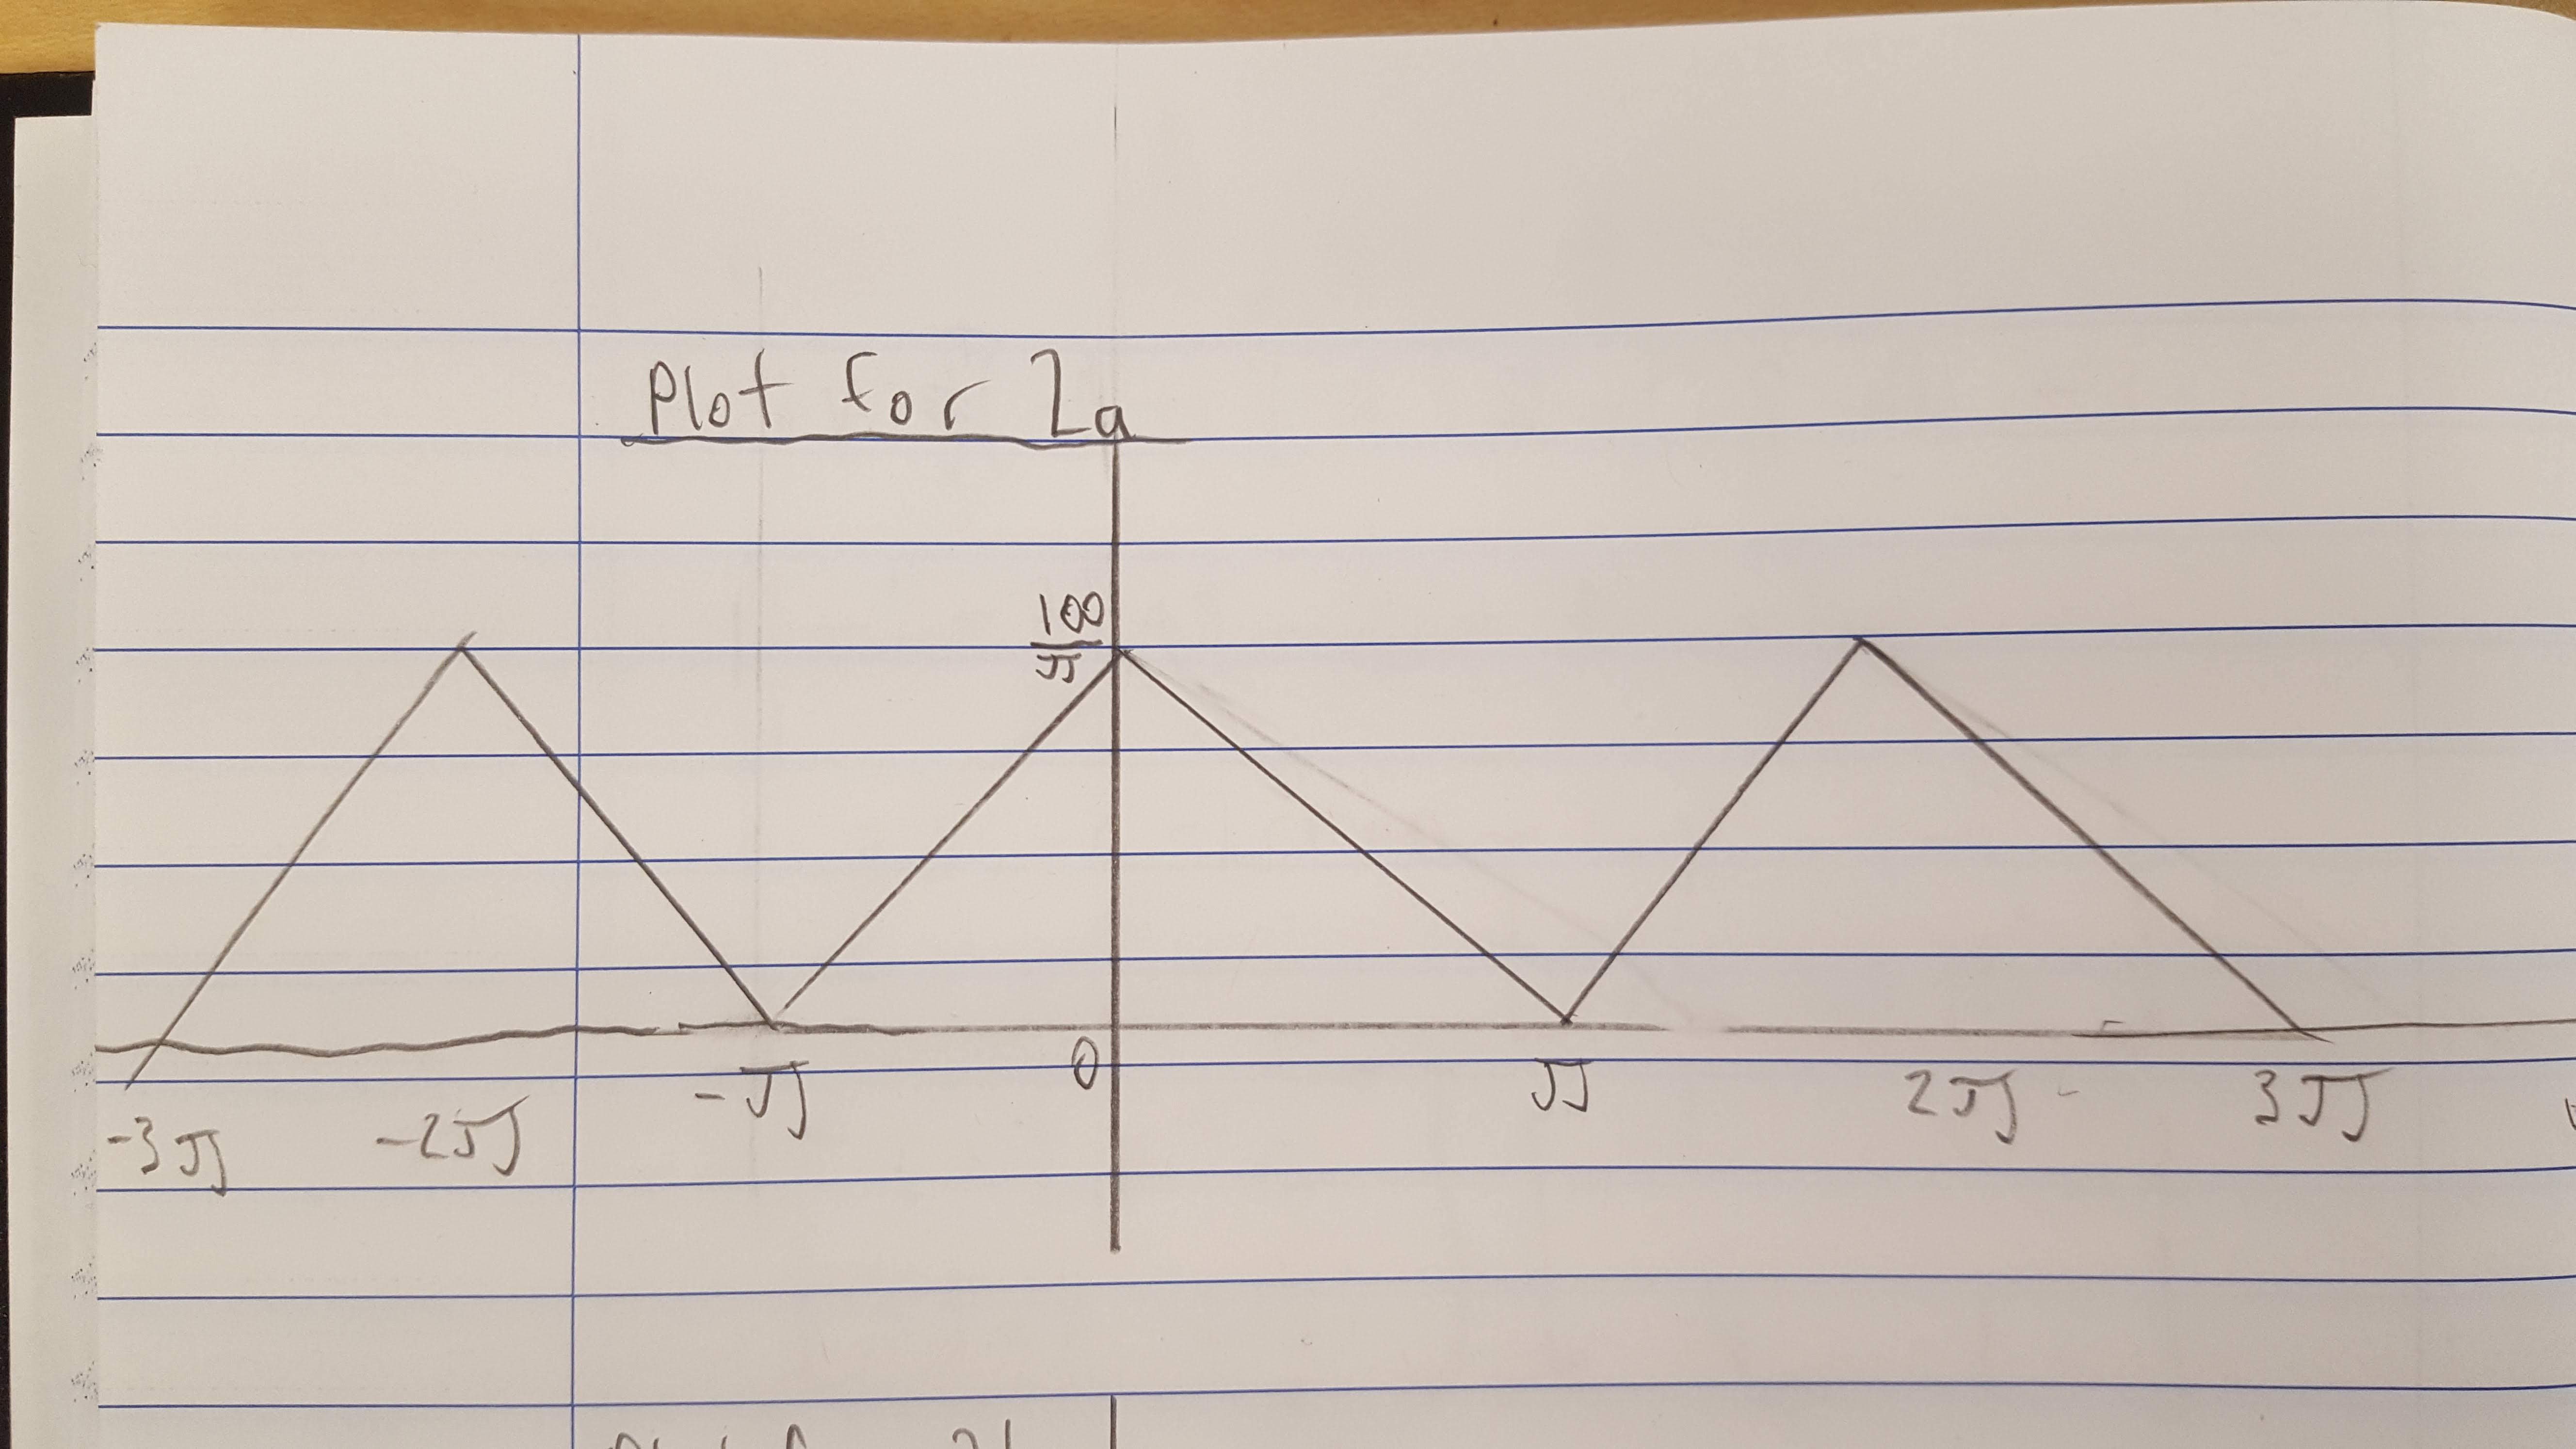
\includegraphics[width=\textwidth]{2a}
\caption{$X_d(e^{j\omega})$ for question 2a. }
\label{fig:2a}
\end{figure}

{\noindent\bf Question 2b.} A low pass filter visually takes a fourier transform and cuts it off at it's given frequency, so the result can intuitively be given as 

\[
    Y_d(e^{j\Omega})=\frac{100}\pi\sum_{n\in\ZZ}\begin{cases}1-|(\Omega-2\pi n)/\pi|&|\Omega-2\pi n|\leq \frac\pi2,\\0&\text{ else}\end{cases}
\]

A graph of this can be seen in figure \ref{fig:2b}. 

\begin{figure}[htbp]
\centering
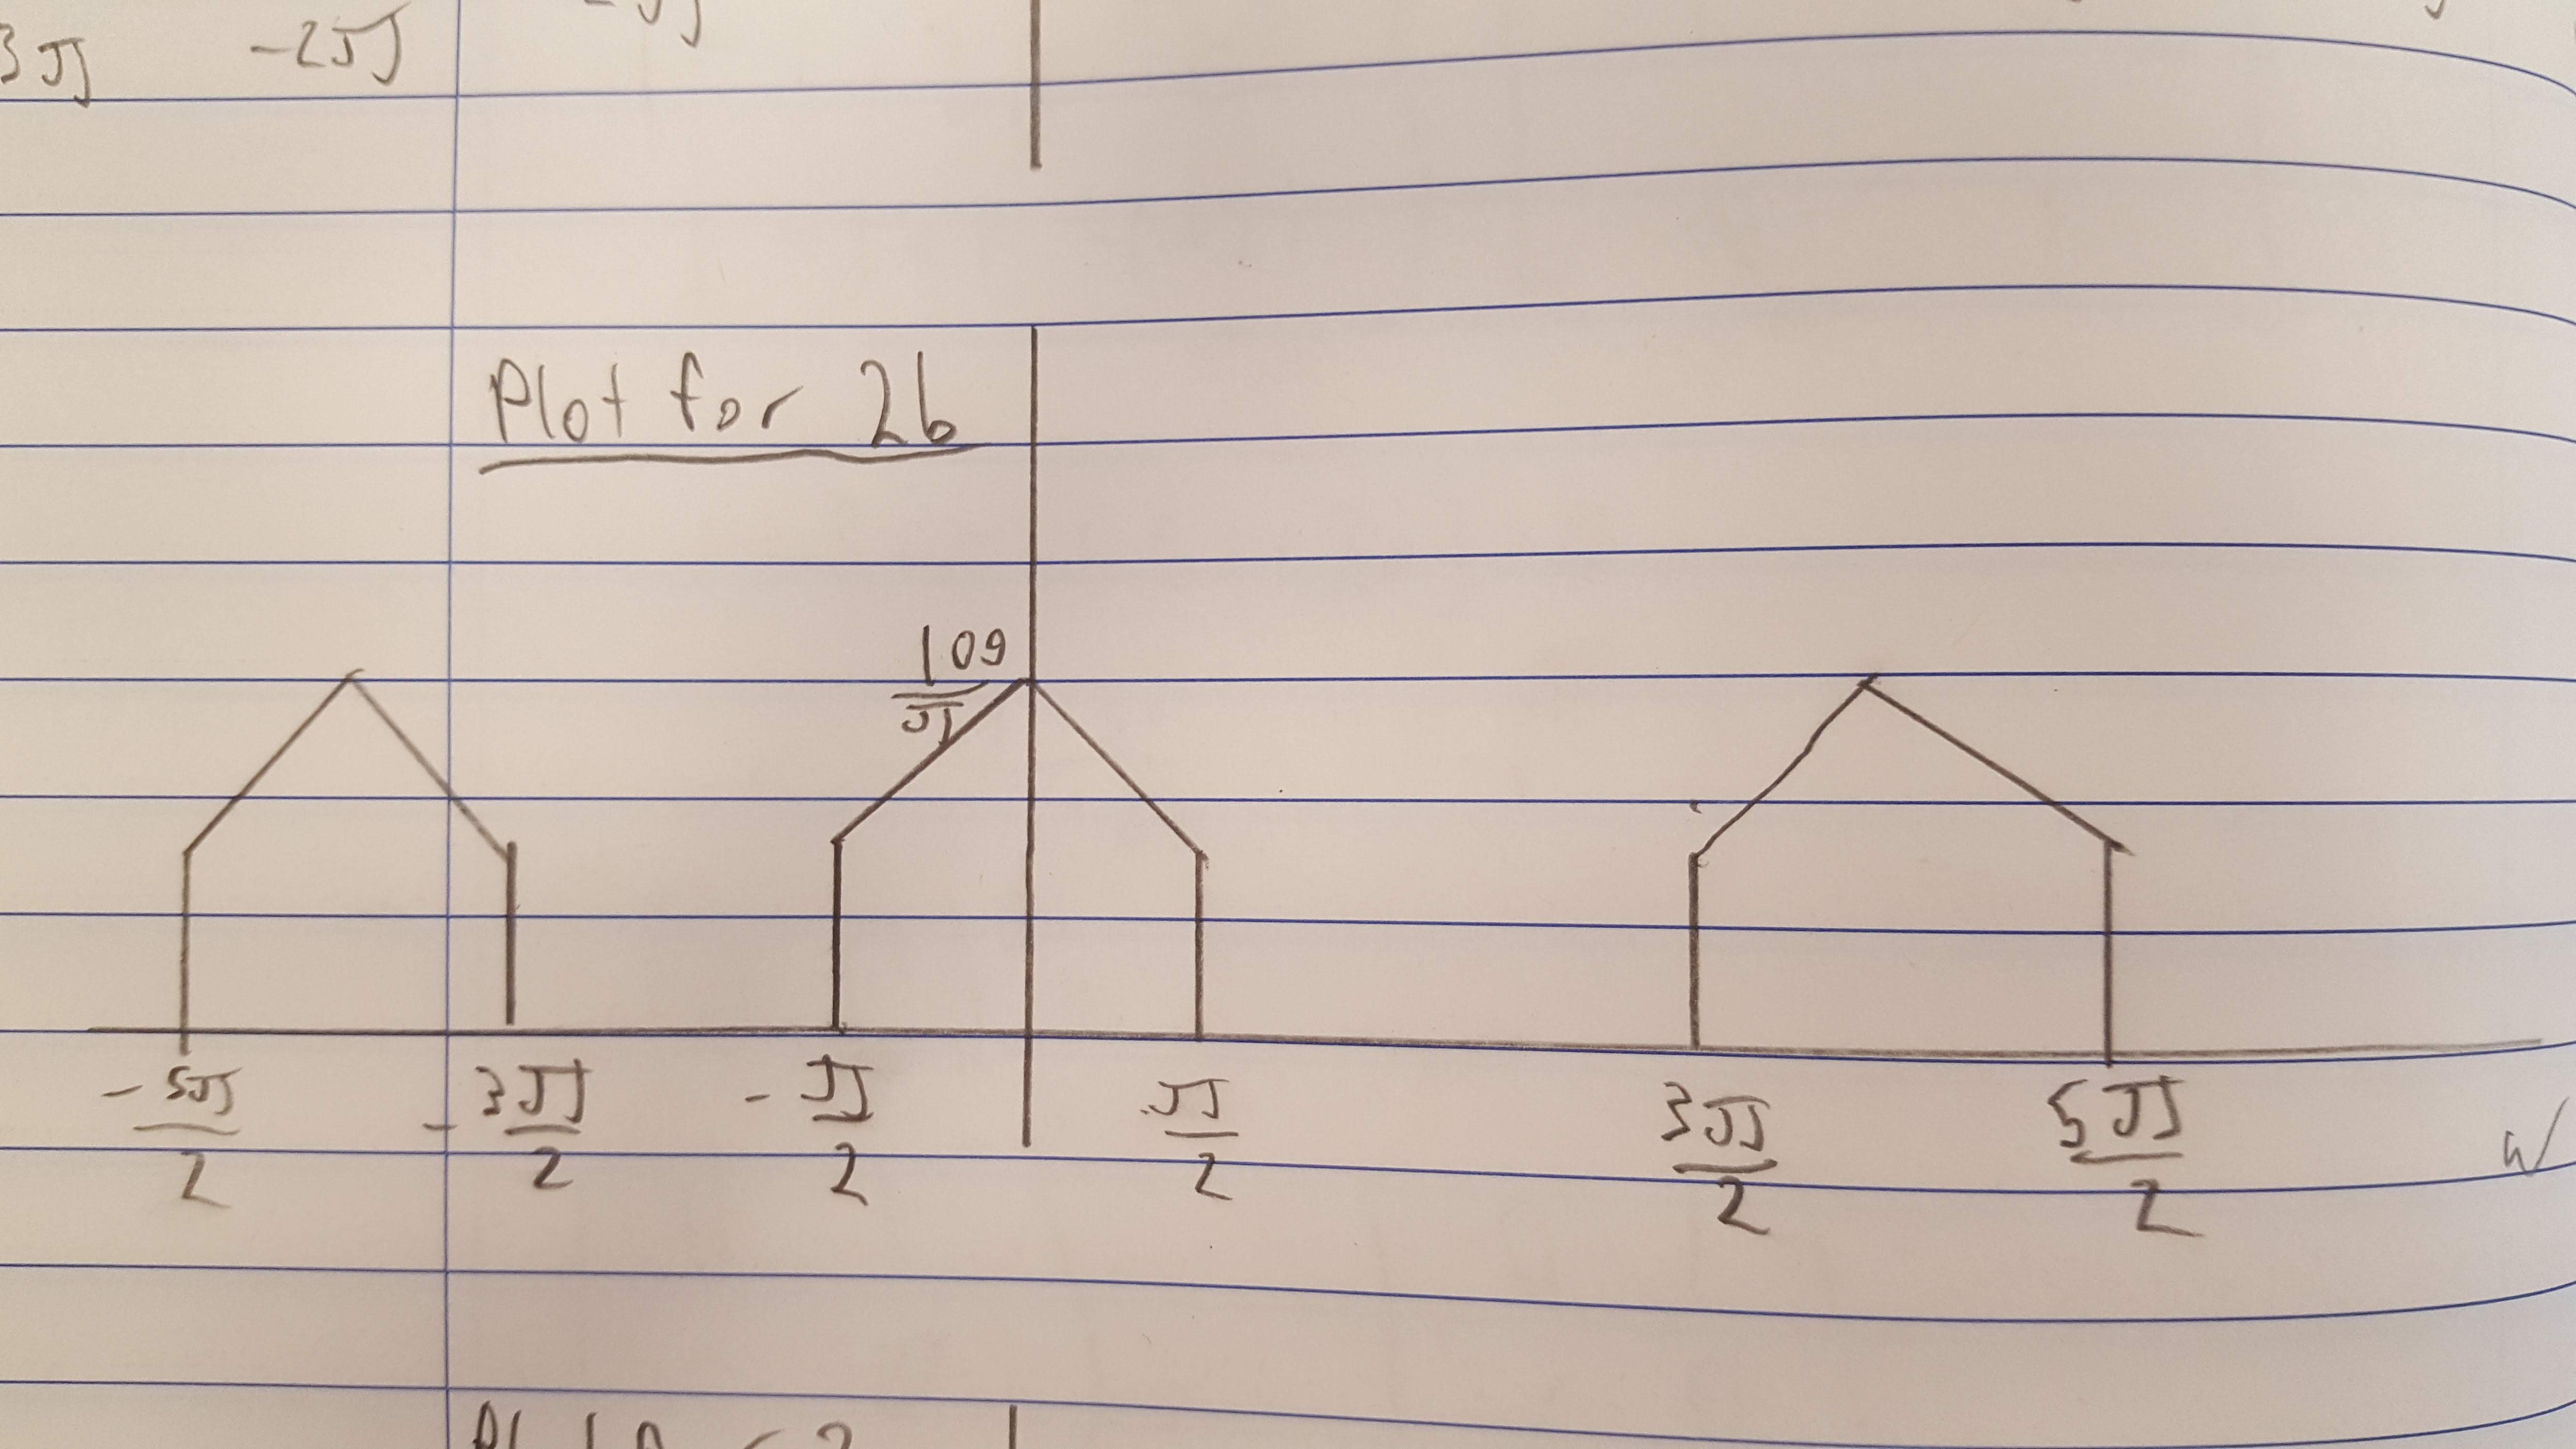
\includegraphics[width=\textwidth]{2b}
\caption{$Y(e^{j\omega})$ for question 2b. }
\label{fig:2b}
\end{figure}

{\noindent\bf Question 2c.} Note that on Piazza this was clarified to actually mean the FT of $y_p(t)$, not $y_c(t)$ so I will answer it as such. We showed in class that for this form of reconstruction, we have that 

\[
    Y_s(j\omega)=Y_d(e^{j\omega T})=\frac{100}\pi\sum_{n\in\ZZ}\begin{cases}1-|(\Omega/100-200 n)|&|\Omega-200 n|\leq 50,\\0&\text{ else}\end{cases}
\]

A graph of this can be seen in figure \ref{fig:2c}. 

% \[
%     Y_s(j\omega)=\frac1T\sum_{n\in\ZZ} X(j(\omega-n\omega_s))\cdot H(e^{j\omega T})
% \]

% Plugging in our known $Y_d(e^{j\omega})$, we get 

% \[
%     Y_s(j\omega)=\frac{100}\pi\sum_{n\in\ZZ} Y_d(e^{j(\omega/100-2n)})
% \]

% This effectively results in an infinite sum of the same graph as in the previous question. A plot of this can be seen in figure \ref{fig:2c}. 

\begin{figure}[htbp]
\centering
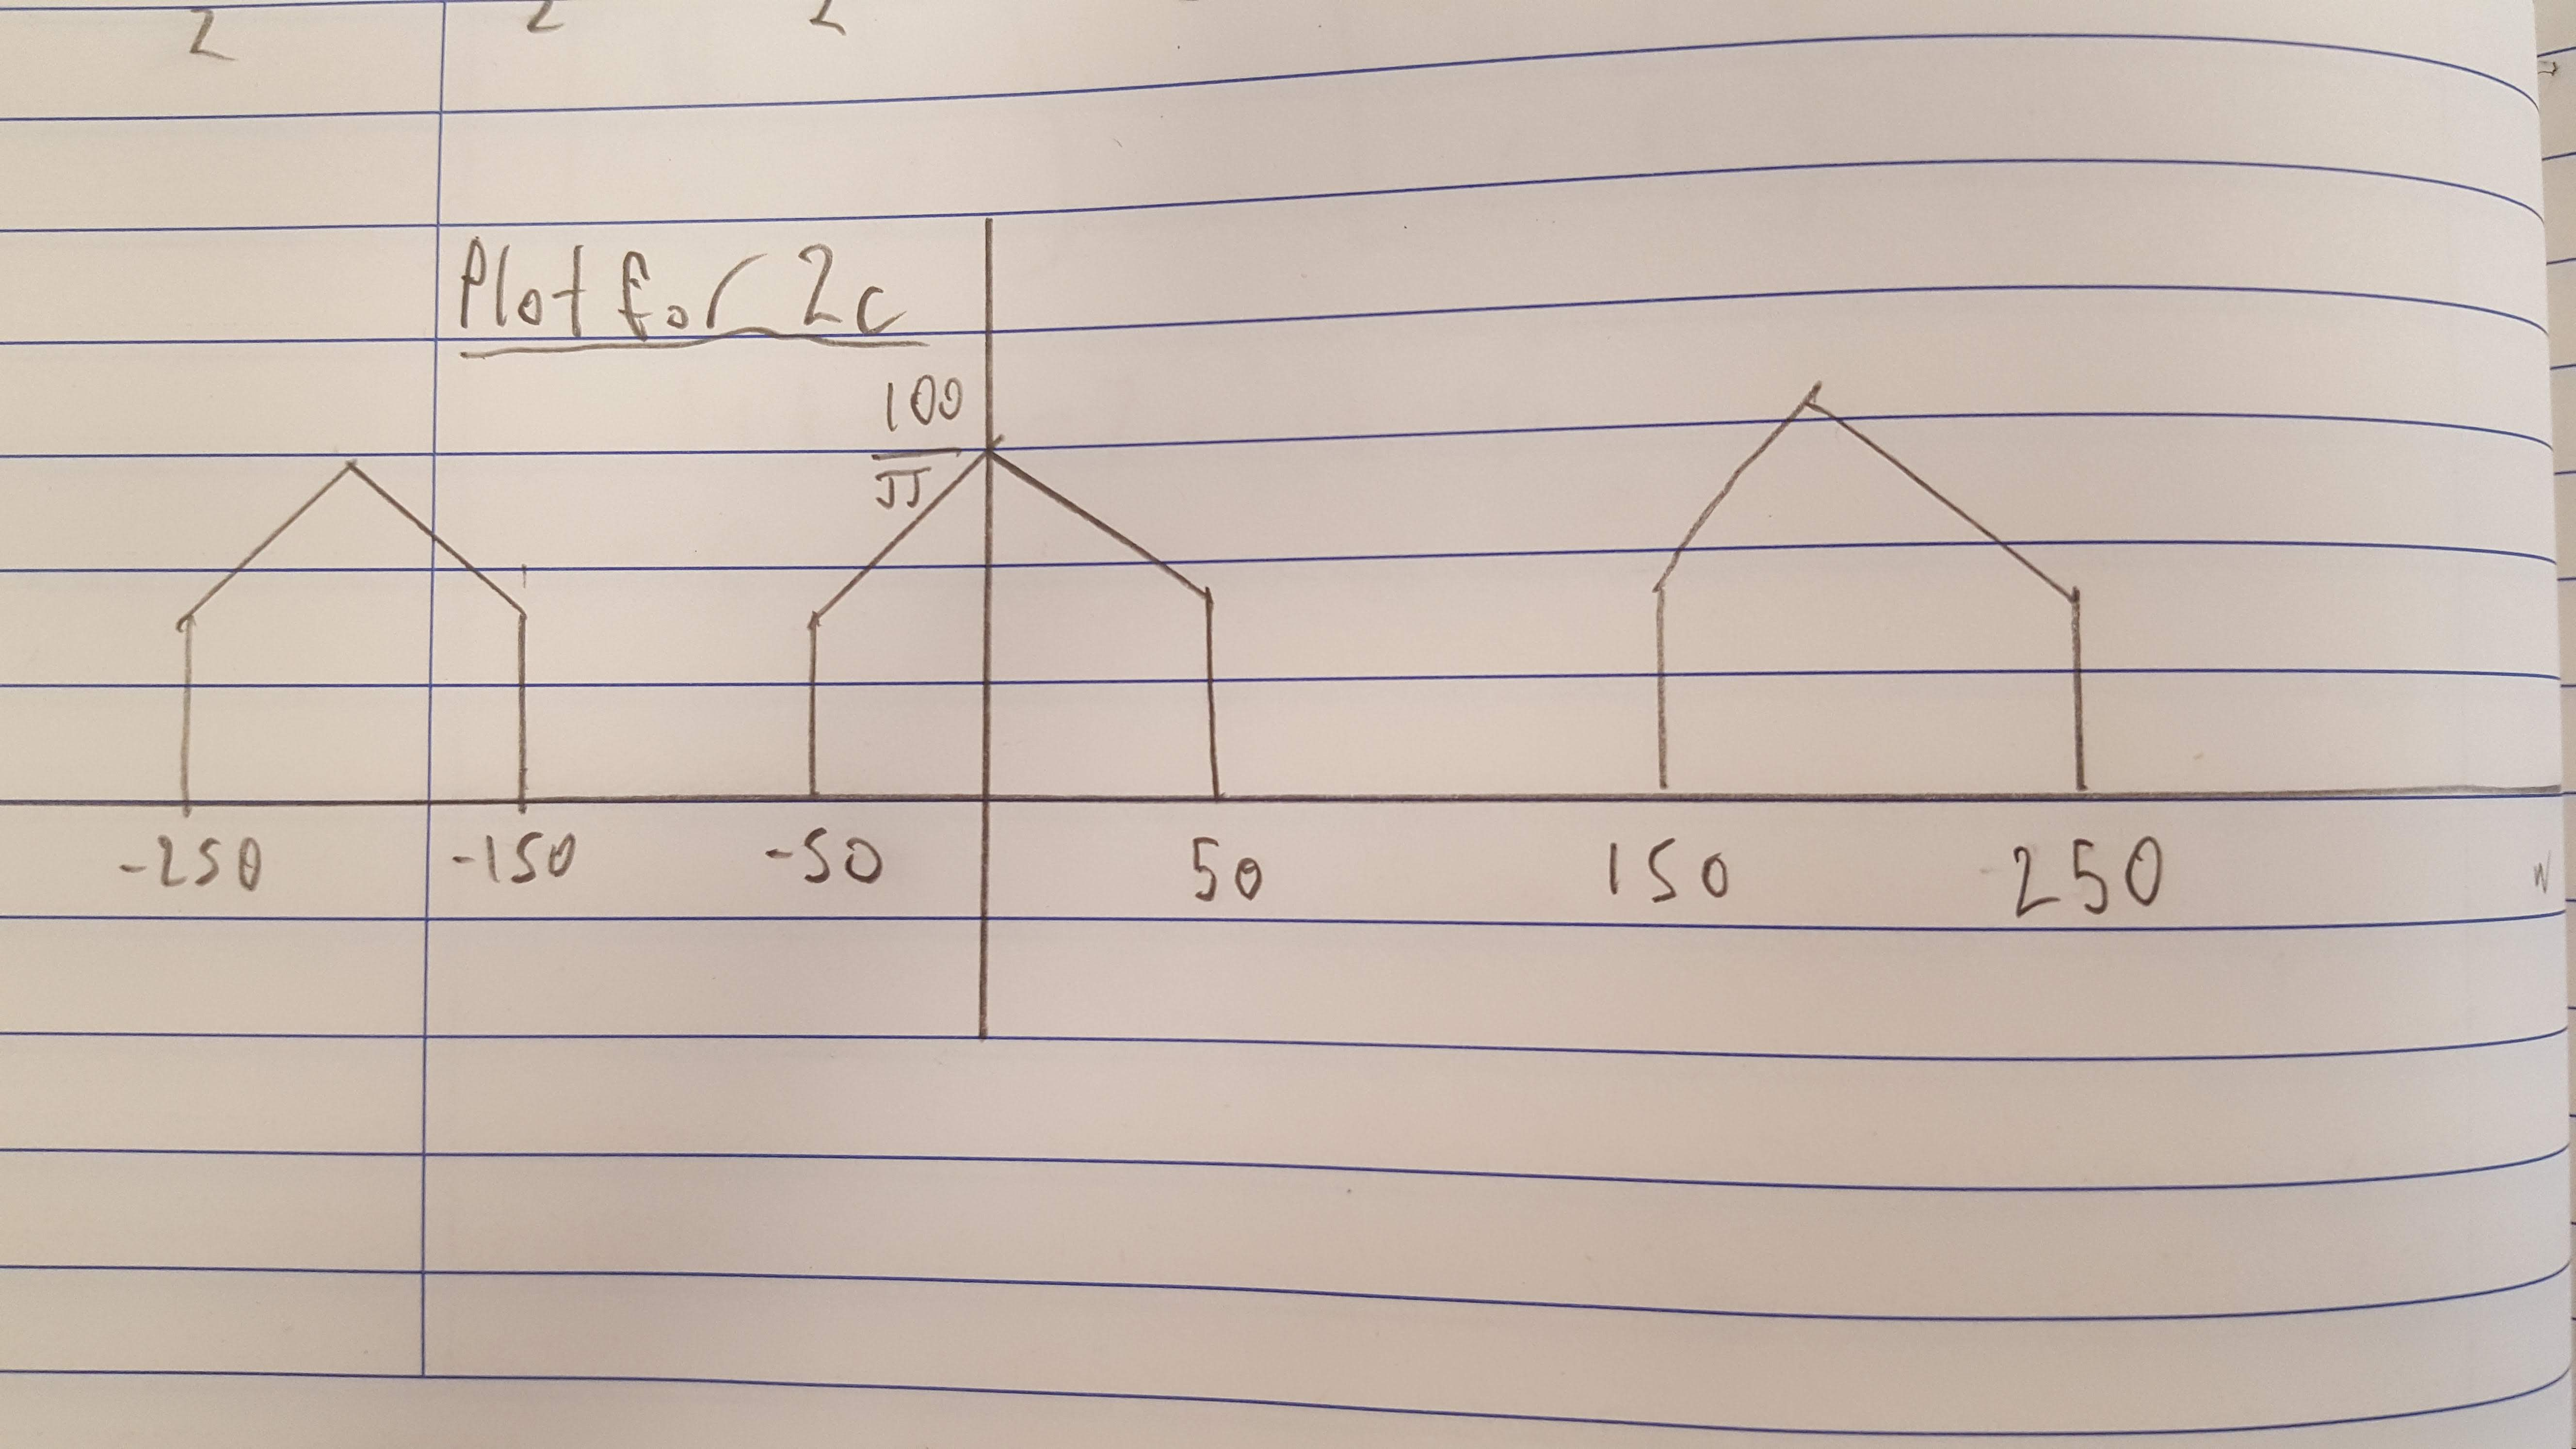
\includegraphics[width=\textwidth]{2c}
\caption{$Y_s(j\omega)$ for question 2c. }
\label{fig:2c}
\end{figure}

{\noindent\bf Question 2d.} The final ideal low pass filter takes in $Y_s(j\omega)$ and gets rid of the periodicity that comes with the infinite sum, and the gain gets rid of the coefficients in front. Thus the final FT output of the system is 

\[
    Y_c(j\omega)=\begin{cases}1-|\omega/100|&|\omega|\leq 50,\\0&\text{ else}\end{cases}
\]

A plot of this can be seen in figure \ref{fig:2d}. Note that this is the original signal, just now band limited and filtered, which makes sense. 

\begin{figure}[htbp]
\centering
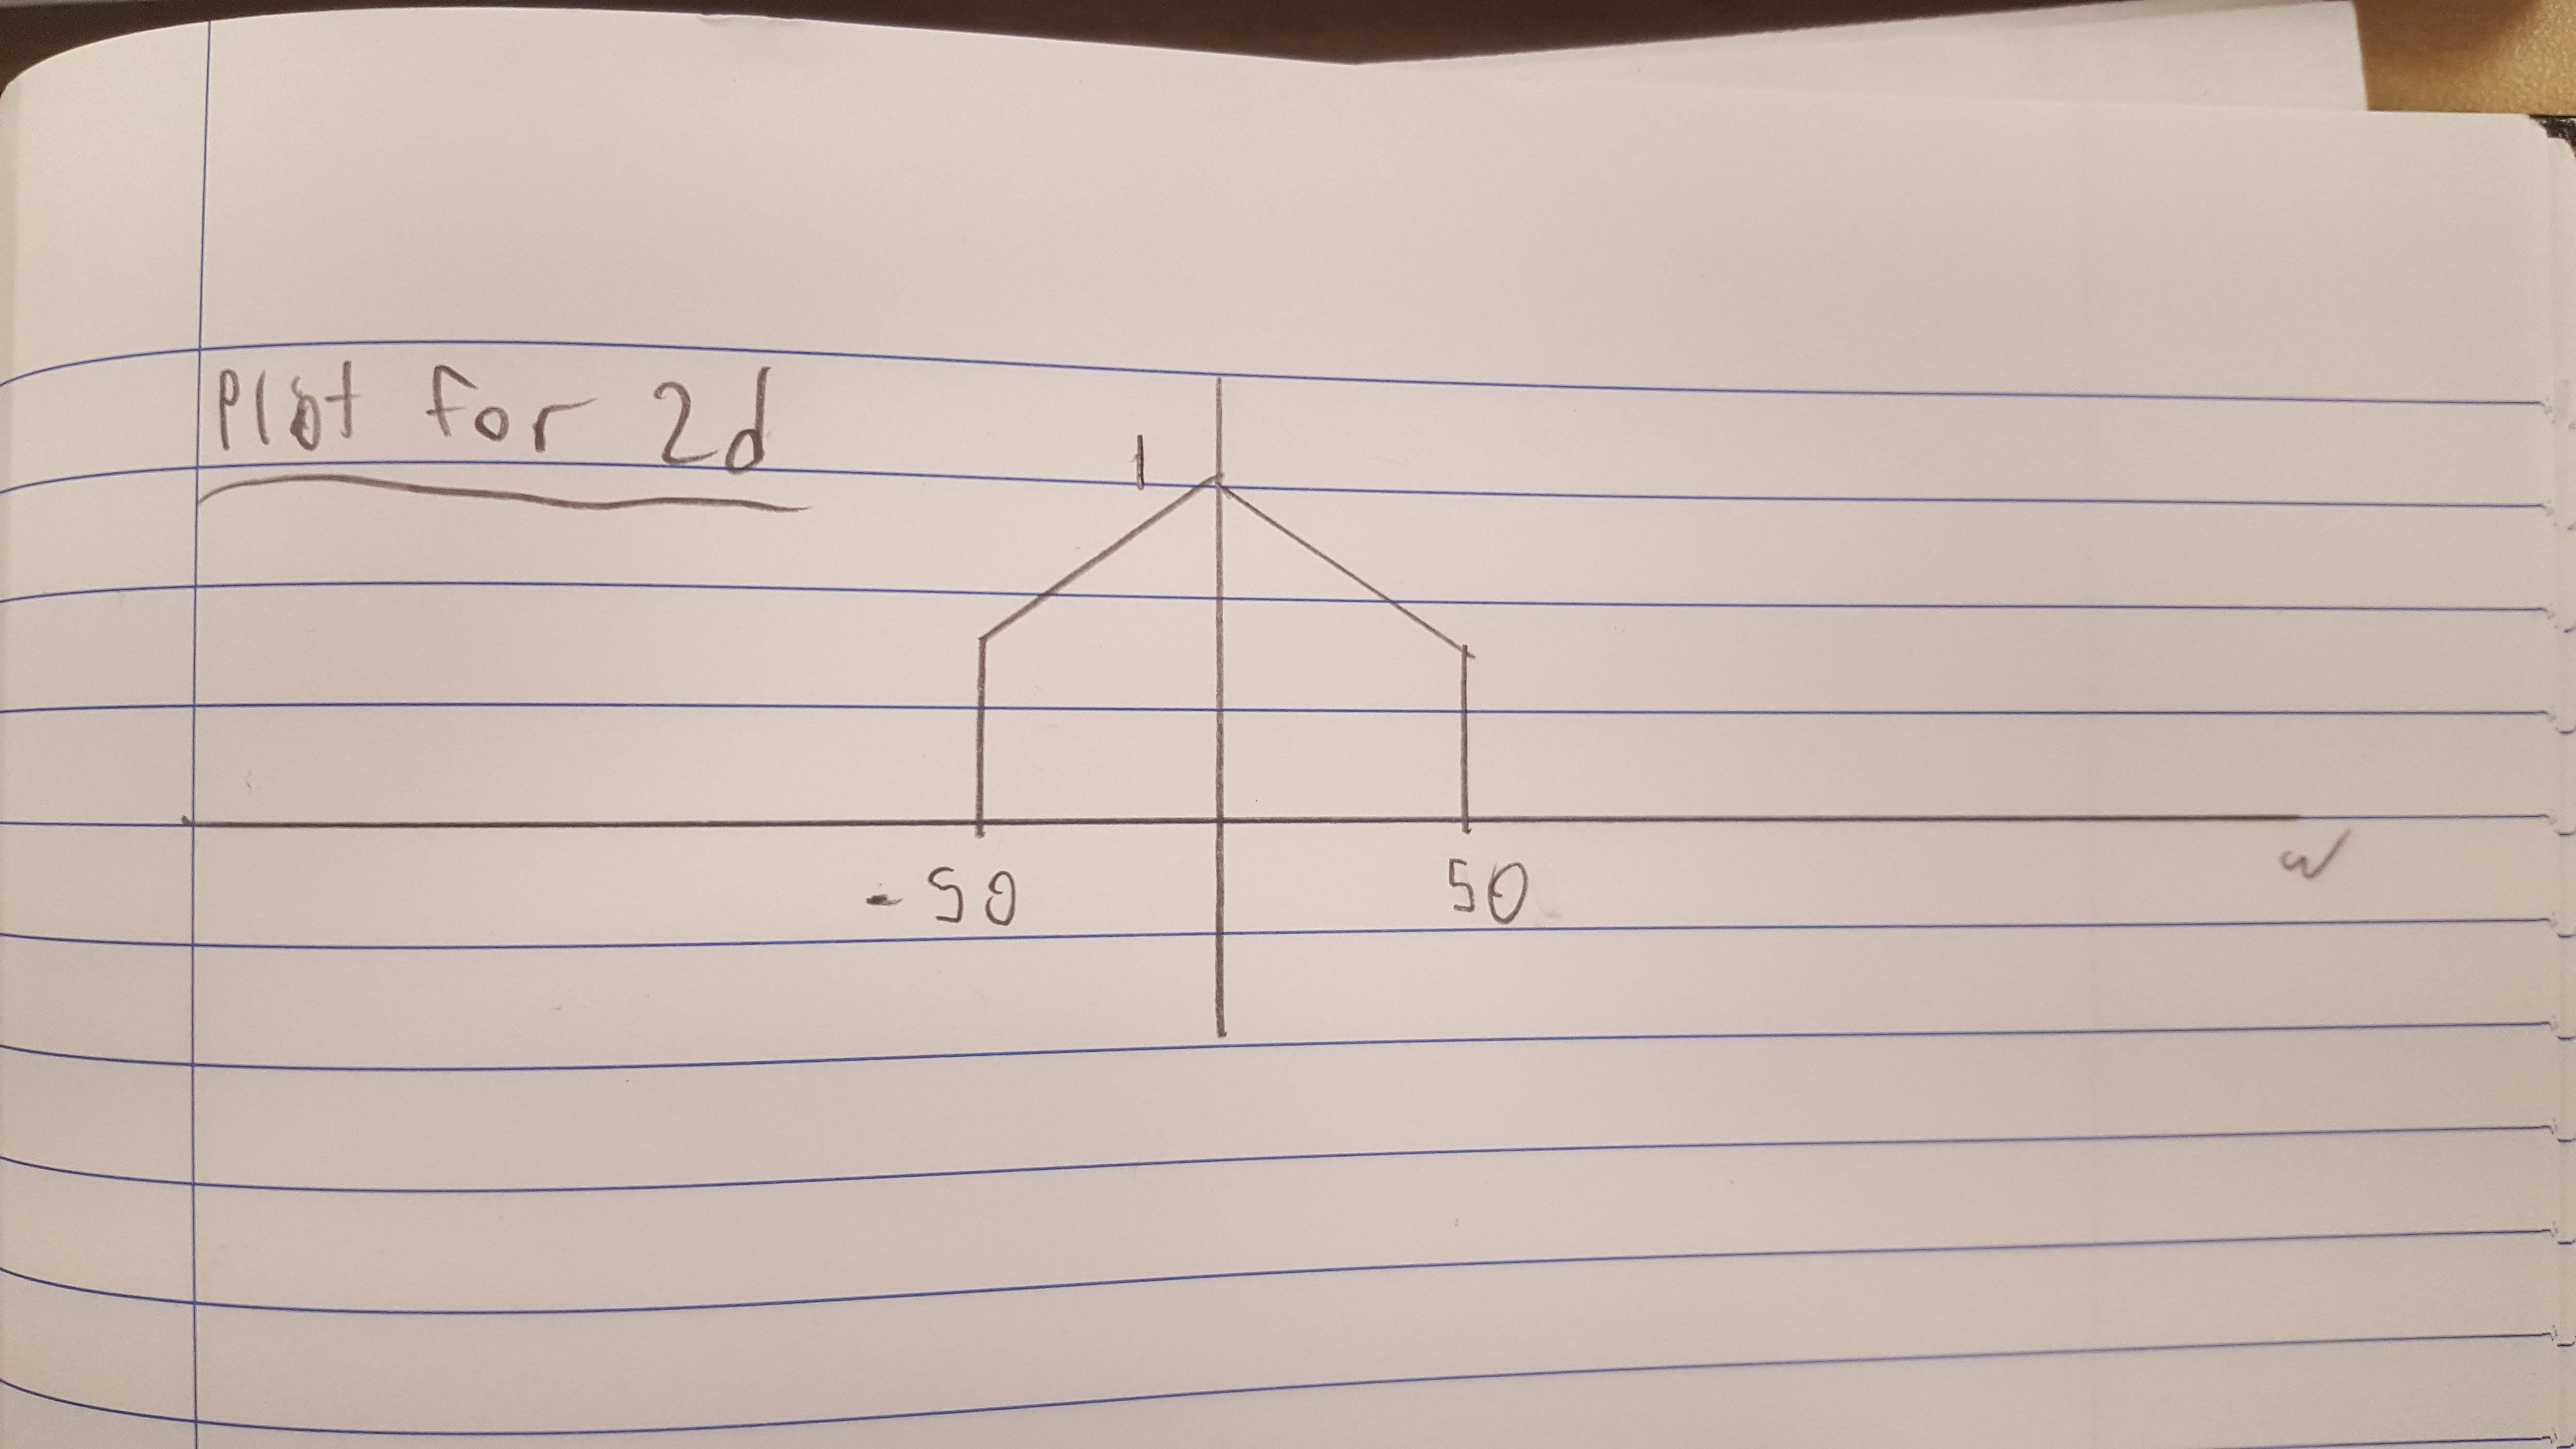
\includegraphics[width=\textwidth]{2d}
\caption{$Y_c(j\omega)$ for question 2d. }
\label{fig:2d}
\end{figure}

{\noindent\bf Question 2e.} Take the DTFT of both sides. Applying the modulation property gives 

\[
    Y(e^{j\omega})=\frac12 e^{-j\omega} Y(e^{j\omega})+X(e^{j\omega})
\]

\[
    H(e^{j\omega}) = \frac{Y(e^{j\omega})}{X(e^{j\omega})}=\frac1{1-\frac12e^{-j\omega}}
\]

The FT of $x_d(t)$, as we found in the previous parts of the question, is 

\[
    X_d(e^{j\Omega}) = \frac1T \sum_{n\in\ZZ}X_c(j\frac{\Omega-2\pi n}T)
\]

The output of the difference equations box would then be the product between the fourier transform of the input and the frequency response, i.e.

\[
    Y_d(e^{j\Omega})=H(e^{j\Omega})X_d(e^{j\Omega})=\frac1T\sum_{n\in\ZZ}\frac{X_c(j\frac{\Omega-2\pi n} T)}{1-\frac12e^{-j\Omega}}=\frac{100}\pi\sum_{n\in\ZZ}\frac{X_c(j\frac{100\Omega-200\pi n} \pi)}{1-\frac12e^{-j\Omega}}
\]

{\noindent\bf Question 2f.} As in part c, we use the identity that 

\[
    Y_p(j\omega)=Y_d(e^{j\omega T})=\frac{100}\pi\sum_{n\in\ZZ}\frac{X_c(j(\omega-200 n))}{1-\frac12e^{-j\frac{100}\pi\omega}}
\]

{\noindent\bf Question 2g.} The last step just band limits this last step, so assuming that $X_c(j\omega)$ is band limited to $W=100$, then we get that 

\[
    Y_c(j\omega) = \frac{X_c(j\omega)}{1-\frac12 e^{-j\frac{100}\pi\omega}}    
\]

\end{document}